\documentclass[a4paper,11pt, twoside]{article}

\usepackage[a4paper,top=3cm,bottom=3.5cm,left=2.5cm,right=2.5cm]{geometry}
\usepackage{graphicx}
\usepackage[utf8]{inputenc}
\usepackage[italian]{babel}
\usepackage{fancyhdr}
\usepackage{amssymb}
\usepackage{makeidx}
\usepackage{eurosym}
\usepackage{hyperref}
\usepackage{varioref}
\usepackage{xmpincl}
\usepackage{ccicons}
\usepackage{subfigure}
\usepackage{amsmath}

\makeatletter
\newcommand{\xRightarrow}[2][]{\ext@arrow 0359\Rightarrowfill@{#1}{#2}}
\makeatother
\usepackage{amsthm}

\theoremstyle{definition}
\newtheorem{defn}{Definizione}[section]

\title{Appunti di Linguaggi Formali e Compilatori}
\author{Matteo Gianello}
\date{\today}

\pdfinfo{%
  /Title    (Appunti di Linguaggi Formali e Compilatori)
  /Author   (Matteo Gianello)
  /Creator  (Matteo Gianello)
  /Producer ()
  /Subject  ()
  /Keywords (Linguaggi Formali e Compilatori IngInf Polimi)
}
\makeindex
\includexmp{licenza}
\begin{document}
\pagestyle{empty}
\thispagestyle{empty}
\maketitle
\vspace{5cm}
\begin{center}
Quest'opera è stata rilasciata con licenza Creative Commons Attribuzione - Non commerciale - Condividi allo stesso modo 4.0 Internazionale. Per leggere una copia della licenza visita il sito web \url{http://creativecommons.org/licenses/by-nc-sa/4.0/}. \ccbyncsa.
\end{center}
\newpage

\thispagestyle{plain}
\tableofcontents
\newpage

\pagestyle{plain}
\section{Introduzione}
Prima di entrare nel dettaglio della nostra trattazione definiamo che cos'è un \emph{Linguaggio Formale.} Innanzitutto dobbiamo distinguere tra un \emph{linguaggio natura} ed uno \emph{artificiale}, un linguaggio naturale è quello che utiliziamo tutti i giorni e che si basa sul significato delle parole e soprattutto non possiede una struttura formale. Un linguaggio artificiale, invece, è quello utilizzato per la comunicazione tra macchine, è di tipo no verbale ma soprattutto è formale.\\
Un linguaggio si definisce \textbf{formale} se la sua \emph{sintassi} (ovvero la sua struttura) e la sua \emph{semantica} (ovvero il suo significato) sono definiti da precisi algoritmi. Questo permette di definire delle \emph{procedure} precise per determinare la correttezza di una frase che appartiene ad un linguaggio e il suo significato. 
In un contesto più ristretto un \textbf{linguaggio formale} è un \emph{oggetto matematico} costruito su di un \emph{alfabeto} tramite regole assiomatiche chiamate \emph{grammatiche} o tramite strumenti matematici chiamati \emph{automi}.\\
\subsection{Introduzione alla teoria dei linguaggi formali}
Vediamo ora alcune definizioni che ci saranno utili durante il corso:
\begin{description}
	\item[Alfabeto:] insieme \emph{finito} di elementi
	$$\Sigma = \{a_1, a_2, a_3, \dots, a_k\}$$
	\item[Cardinalità di un alfabeto:]  è il numero di elementi che lo compongono
	$$ |\Sigma| = k $$
	\item[Stringa:] insieme ordinato di elementi dell'alfabeto che possono essere anche ripetuti.
	$$\Sigma = \{a,b,c\}$$
	$$Stringe: \ abc \vee aab \vee ac \vee bbb$$
	\item[Linguaggio:] insieme finito o infinito di stringhe di un alfabeto
	$$L_1 = \{ab,ac,abc\}$$
	$$L_2 = \{bc,bbc,\dots\}$$
	La struttura insiemistica del linguaggio formale ha due livelli di profondità:
	\begin{itemize}
		\item Insieme non ordinato di elementi non atomici (\emph{stringhe}) che sono
		\item sequenze ordinate di elementi atomici (\emph{elementi o terminali}).
	\end{itemize}
	\item[Cardinalità di un linguaggio:] può essere finita o infinita.
	$$|L_1| = |\{ab,ac,abc\}| = 3$$
	\item[Lunghezza di una stringa:] indica il numero dei suoi elementi
	$$|abb| = 3 \quad |abbc| = 4$$
	\item[Uguaglianza tra stringhe:] due stringhe si definiscono uguali se e solo se hanno la stessa lunghezza, ed i suoi elementi coincidono ordinatamente da sinistra a destra.
	$$x = a_1a_2\dots a_h \quad y = b_1b_2\dots b_k$$
	$$x = y \iff h = k \wedge a_i = b_i \ \forall i = 1\to h $$
\end{description}
\subsubsection{Operazioni con le stringhe}
La \emph{concatenazione} è l'operazione fondamentale con le stringhe, si tratta di fare il prodotto tra esse. Questa operazione è un operazione di base e non fa altro che disporre in fila le due stringhe.
$$x = a_1a_2\dots a_h \quad y = b_1b_2\dots b_k$$
$$x\cdot y = a_1a_2\dots a_hb_1b_2\dots b_k = xy$$
Questo tipo di operazione gode della proprietà associativa e va ad influire sulla lunghezza della stringa come vediamo dalla \ref{eq:conass} e dalla \ref{eq:conlen}.
\begin{equation}\label{eq:conass}
	(xy)z = x(yz)
\end{equation}
\begin{equation}\label{eq:conlen}
	|xyz| = |x| + |y| + |z|
\end{equation}
La concatenazione ci permette di introdurre un altro concetto relativo alle stringhe, ovvero quello della \emph{stringa vuota} o \emph{nulla} indicata con $ \varepsilon $ questa stringa è l'elemento neutro rispetto all'operazione di concatenazione, infatti, concatenando $ \varepsilon $ a destra o a sinistra di una stringa la stringa non cambia.
$$\varepsilon x = x\varepsilon = x$$
Tuttavia bisogna prestare attenzione a non confondere la stringa nulla con l'insieme vuoto $Phi$.\\
Una volta capita l'operazione di concatenazione si possono individuare in una stringa delle \emph{sotto-stringhe}, ovvero stringhe più piccole concatenate tra loro per formare una stringa più grande.
Ad esempio data una stringa $x$ essa può essere vista come un insieme di sotto-stringhe concatenate
$$x = uyv$$
Dove:
\begin{itemize}
	\item \emph{y} è detta sotto-stringa.
	\item \emph{u} è chiamato prefisso.
	\item \emph{v} è chiamato suffisso.
\end{itemize}
Un esempio di suffissi, prefissi e sotto-stringhe è mostrato in \figurename\,\ref{fig:sufpref}.
\begin{figure}
	\centering
	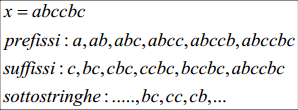
\includegraphics[width=0.5\linewidth]{img/substr.png}
	\caption{Esempio di sottostringhe con prefissi e suffissi}\label{fig:sufpref}
\end{figure}

Si definiscono \emph{sotto-stringhe proprie} tutte quelle stringhe che hanno $u\neq \varepsilon$ e $v \neq \varepsilon$
\section{Linguaggi ed espressioni regolari}
I \emph{linguaggi regolari} sono la famiglia più semplice di linguaggi formali, questo perché possono essere definiti in diversi modi:
\begin{itemize}
	\item Algebricamente.
	\item Attraverso grammatiche generative.
	\item Attraverso algoritmi di riconoscimento (\emph{automi})
\end{itemize}
Le \emph{espressioni regolari} (\emph{regexp}) sono stringhe \emph{r} definite attraverso i caratteri di un alfabeto $ \Sigma $ e mediante l'utilizzo dei meta-simboli $ \varnothing, \cup, \cdot, \ast $ attraverso l'applicazione e la combinazione delle seguenti regole
\begin{itemize}
	\item $ r= \varnothing $
	\item $ r = a, a\in \Sigma $
	\item $ r = (s \cup t) $
	\item $ r = (s\cdot t) \ o \ r = (st) $
	\item $ r = (s)^\ast $
\end{itemize}
Oltre a questi simboli talvolta, per semplificare la notazione, si utilizzano anche i simboli $ \varepsilon = \varnothing^\ast$ e $ r^+ = e\cdot e^\ast $.\\
Il risultato di un'espressione regolare \emph{e} è un linguaggio $ L_e $ costruito sull'alfabeto $ \Sigma $ che rispecchia le regole di \tablename\ref{tab:reggen}
\begin{table}
	\centering
\begin{tabular}{|c|c|}
	\hline \textbf{regexp} & \textbf{Linguaggio} \\ 
	\hline $ \varepsilon $ & $ \{\varepsilon\} $ \\ 
	\hline $ a\in\Sigma $ & $ \{a\} $ \\ 
	\hline $ s\cup t $ & $ L_s \cup L_t $ \\ 
	\hline $ s\cdot t $ & $ L_s\cdot L_t $ \\ 
	\hline $ s^\ast $ & $ L_s^\ast $ \\ 
	\hline 
\end{tabular}
\caption{Regole di generazione dei linguaggi da regexp}\label{tab:reggen}
\end{table}
A questo punto possiamo dire che un linguaggio è \emph{regolare} se è generato tramite l'utilizzo di \emph{espressioni regolari} come ad esempio
$$ e = (111)^* \quad L_e=\{1^{3n}|n = 0,1,\dots \} $$
\subsection{La famiglia dei linguaggi regolari}
Definiamo la \emph{famiglia dei linguaggi regolari} (\texttt{REG}) come la collezione di tutti i linguaggi regolari, inoltre, definiamo la \emph{famiglia dei linguaggi finiti} (\texttt{FIN}) la collezione di tutti i linguaggi aventi \emph{cardinalità finita}.\\
Ogni linguaggio finito è regolare in quanto è l'unione ($ \cup $) di un numero finito di stringhe le quali sono il concatenamento ($ \cdot $) di un numero finito di caratteri. Tuttavia l'insieme dei linguaggi regolari contiene anche linguaggi non finiti perciò l'inclusione risulta essere stretta.
$$FIN\subset REG$$
\subsection{Sottoespressione di un'espressione regolare}
Consideriamo un espressione completamente parentesizzata come la seguente:
$$e = (a \cup (bb))^\ast(c^+\cup(a \cup (bb)))$$
A questo punto distinguiamo tutti i termini numerandoli
$$e = (a_1 \cup (b_2b_3))^\ast(c_4^+\cup(a_5 \cup (b_6b_7)))$$
Infine mettiamo in evidenza tutte le sotto espressioni come mostrato in \figurename\ref{fig:scompo}
\begin{figure}
	\centering
	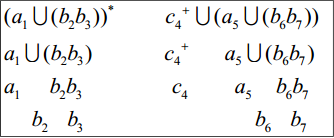
\includegraphics[width=0.5\linewidth]{img/scompo.png}
	\caption{Scomposizione in sottoespressioni}\label{fig:scompo}
\end{figure}
Gli operatori di unione e di ripetizione all'interno di un'espressione regolare corrispondono a possibili alternative o \emph{scelte}, in quanto scegliendo una delle alternative e sostituendola nell'espressione regolare di partenza si ottiene una sottoespressione che definisce un linguaggio più piccolo dell'originale. Le possibile scelte sono elencate in \tablename \ref{tab:scelte}.
\begin{table}
	\centering
	\begin{tabular}{|c|c|}
		\hline
		\textbf{Scelta} & \textbf{Operazione} \\
		\hline
		$ e_k, 1\leq k \leq n $ & $ e_1 \cup e_2 \cup \dots \cup e_n $\\
		\hline
		$ e $ & $ e^*,e^+,e^n $\\
		\hline
		$ \varepsilon $ & $ e^\ast $ \\
		\hline
	\end{tabular}
	\caption{Possibile scelte per le sotto espressioni}\label{tab:scelte}
\end{table}
Data un espressione di partenza $ e_1 $ è sempre possibile derivare una espressione $ e_2 $ sostituendo una sottoespressione con una delle possibili scelte.\\
In termini più matematici definiamo questo processo come:
$$e'\Rightarrow e''$$
dove $ e' $ e $ e'' $ sono definite come:
$$e' = \alpha\beta\gamma \quad e'' = \alpha\delta\gamma$$
dove $ \beta $ è una sottoespressione regolare di $ e' $ e $ \delta $ è sottoespressione regolare di $ e'' $ ed inoltre $ \delta $ è una scelta di $ \beta $. Questo processo di derivazione può essere applicato in sequenza più volte.
$$
\begin{array}{ccc}
e_0\xRightarrow{n} e_n &e_0\Rightarrow e_1\dots&e_{n-1}\Rightarrow e_n\\
e_0 \xRightarrow{\ast} e_n & e_0 \text{ deriva } e_n & in \ n\geq 0 \ passi\\
e_0 \xRightarrow{+} e_n & e_0 \text{ deriva } e_n & in \ n\geq 1 \ passi
\end{array}$$
Alcune espressioni che si ottengono dalla derivazione di un'\emph{espressione regolare} contengono dei meta-simboli (operatori e parentesi), altre, invece contengono solamente i simboli dell'alfabeto $ \Sigma $ e la lettera $ \varepsilon $ questi simboli sono detti \emph{terminali}.
Questo tipo di derivazioni costituiscono il linguaggio definito dall'espressione regolare di partenza. Il linguaggio generato da una determinata \emph{regexp} di partenza $ r $ è definito come:
$$L(r) = \{x \in \Sigma^\ast | r \xRightarrow{\ast} x \}$$
Un linguaggio generato da un'espressione regolare derivata è contenuto nel linguaggio generato dall'espressione regolare di partenza. Due \emph{regexp} si definiscono equivalenti se \emph{generano} lo stesso linguaggio. Possono esistere diverse derivazioni che portano alla stessa stringa, queste derivazioni risultano essere equivalenti.\\
Alcune volte, è possibile, che due stringhe equivalenti siano ottenute dallo stesso linguaggio non solo cambiando l'ordine di derivazione ma più in generale tramite una differenza strutturale, in questo caso si parla di \emph{ambiguità} dell'espressione regolare.\\
Una regexp $ f $ si definisce \emph{ambigua} se la sua versione numerata $ f' $ genera due stringhe $ x $ e $ y $ tali che queste due stringhe, private della numerazione, coincidono. Ad esempio l'espressione 
$$f'= (a_1\cup b_2)^\ast a_3 (a_4 \cup b_5)^\ast$$
Può generare le due stringhe $a_1a_3$ e $a_3a_4$
\subsection{Altre operazioni con le espressioni regolari}
Oltre a ciò che abbiamo già visto alle espressioni regolari possiamo applicare l'operatore \emph{potenza} $a^h = aaa\dots \ h-volte$, l'operatore \emph{ripetizione} che si indica come:
$$[a]_k^n = a^k\cup \dots \cup a^n$$
L'\emph{opzionalità}, indicata come:
$$[a] = (\varepsilon \cup a)$$
e l'\emph{intervallo ordinato} indica un insieme ordinato di simboli come ad esempio $(0\dots 9)$.
Inoltre, nelle espressioni regolari possiamo utilizzare le operazioni insiemistiche (intersezione, differenza e complemento), tuttavia l'utilizzo di quest'ultime non aumenta la potenza espressiva delle espressioni regolari ma serve solo ad abbreviare la notazione. Quando si utilizzano le operazioni insiemistiche si parla di \emph{espressioni regolari estese}.
Un esempio di questo tipo di operazioni è l'\emph{intersezione} che esprime la richiesta della stringa di soddisfare due richieste contemporaneamente come ad esempio:
$$r = (a|b)^*bb(a|b)^*\cap ((a|b)^2)^*$$
Che indica una stringa che contiene almeno i caratteri $ bb $ e che la lunghezza della stringa sia pari. Questa richiesta risulta essere più complessa nel caso non si utilizzino le operazioni insiemistiche come si vede dalla seguente formula che esprime la stessa richiesta precedente:
$$((a|b)^2)^*bb((a|b)^2)^*|(a|b)((a|b)^2)^*bb(a|b)((a|b)^2)^*$$
\subsection{Chiusura dei linguaggi regolari rispetto alle operazioni}
Consideriamo un operatore $ \theta $ che produce un linguaggio (risultato) quando viene applicato a un linguaggio o ad una coppia di linguaggi. Una famiglia di linguaggi si dice chiusa rispetto all'operatore $ \theta $ se il linguaggio risultante appartiene alla stessa famiglia dei linguaggi di partenza.\\
In particolare la famiglia dei linguaggi regolari  è chiusa rispetto agli operatori \emph{unione}, \emph{concatenazione} e \emph{stella}, inoltre per come sono definite le espressioni regolari, la famiglia è chiusa rispetto all'operatore \emph{croce} e \emph{potenza}.\\
Da questa proprietà ne deriva che qualsiasi linguaggio regolare può essere combinato con un altro linguaggio regolare tramite uno degli operatori precedenti ed il risultato sarà un altro linguaggio regolare.
L'\emph{astrazione} di un linguaggio parte da frasi di un linguaggio reale e le trasforma in forme più semplici chiamate \emph{rappresentazioni astratte}. Per fare questo i simboli dell'alfabeto reale vengono sostituiti da quelli dell'alfabeto astratto.\\
A livello di astrazione la struttura di molti linguaggi artificiali può essere ottenuta tramite la composizione di pochi elementi e l'utilizzo di operatori base come l'unione la concatenazione e l'iterazione.

\section{Grammatiche libere}
Fino ad ora abbiamo visto i linguaggi regolari che sono quelli che vengono generati da espressioni regolari. Questo tipo di linguaggi tuttavia risulta essere limitato per rappresentare alcuni linguaggi come ad esempio il seguente:
$$L_1 = {x | x 0 b^ne^n, n\geq 1}$$
Questo linguaggio non è regolare in quanto non esiste un espressione regolare che lo generi. Questo tipo di linguaggi è chiamato \emph{libero dal contesto} e viene generato da \emph{grammatiche libere dal contesto} o più semplicemente \emph{grammatiche libere}.\\
La \emph{sintassi} è lo strumento utilizzato per definire tali linguaggi, essa utilizza delle \emph{regole} le quali, dopo essere state applicate anche ripetutamente, generano tutte e sole le stringhe di tale linguaggio.
L'insieme di queste regole è chiamata \emph{grammatica generativa}.\\
Un esempio di grammatica generativa è quella che genera il linguaggio che contiene l'insieme di stringhe palindrome:
$$L = \{uu^R | u \in \{a,b \}^*\} = \{\varepsilon,aa,bb,abba,baab,\dots\}$$
Generato dall'insieme seguente di regole:
$$
\begin{array}{ccl}
frase & \rightarrow & \varepsilon\\
frase & \rightarrow & a \ frase \ a \\
frase & \rightarrow & b \ frase \ b \\
\end{array}
$$
Una possibile catena di derivazione potrebbe essere
$$frase \Rightarrow a \ frase \ a \Rightarrow ab \ frase \ ba \Rightarrow abb \ frase \ bba \Rightarrow abb\varepsilon bba = abbbba$$
Notiamo come il meta-simbolo $ \rightarrow $ serva a separare la parte sinistra di una regola della grammatica dalla parte destra.\\
Un altro esempio sono le espressioni regolari, le quali definiscono linguaggi regolari tramite l'alfabeto \emph{terminale} $ \Sigma = \{a,b\}$,  sono anch'esse dei linguaggi e in particolare sono definite sull'alfabeto $ \Sigma_{e.r.} = \{a,b,\cup, \ast, \varnothing, (, ) \} $. La sintassi che genera la grammatica $ G_{r.e.} $ è:
$$\begin{array}{llcl}
1. & espr & \rightarrow & \varnothing \\
2. & espr & \rightarrow & a \\
3. & espr & \rightarrow & b\\
4. & espr & \rightarrow & (espr\cup espr) \\
5. & espr & \rightarrow & (espr \ espr) \\
6. & espr & \rightarrow & (espr)^* \\
\end{array}$$
Una grammatica libera dal contesto (nella \emph{forma normale di Backus}) è definita da quattro entità:
\begin{itemize}
\item $ V $ alfabeto di simboli \emph{non terminali}
\item $ \Sigma $ alfabeto dei simboli \emph{terminali}
\item $ P $ insieme di regole \emph{sintattiche} anche chiamato regole di produzione
\item  $ S \in V $ particolare simbolo non terminale chiamato \emph{assioma}.
\end{itemize}
Ogni insieme di regole di $ P $ è una coppia ordinata $ (X,\alpha), X \in V $ e $ \alpha\in(V\cup\Sigma) $. Per evitare confusioni è utile che i meta-simboli $ \rightarrow, | , \cup, \varepsilon $ non siano presenti negli alfabeti $ V $ e $ \Sigma $, inoltre gli alfabeti terminali e non terminali devono essere disgiunti.\\
Introduciamo ora alcune convenzioni, la prima che vediamo è quella per la rappresentazione dei simboli terminali e non terminali, in realtà esistono diversi modi per fare questa distinzione:
\begin{itemize}
	\item utilizzo delle parentesi angolari per i non terminali
	$$<if\_phrase> \rightarrow if <cond> then <prhase> else <prhase>$$
	\item utilizzo del grassetto per i terminali
	$$if\_phrase \rightarrow \text{\textbf{if }} cond \text{\textbf{ then }} prhase \text{\textbf{ else }} prhase$$
	\item utilizzo dei caratteri maiuscoli e minuscoli
	$$ F \rightarrow if \ C \ then \ D \ else \ D $$
\end{itemize}
La convenzione che useremo maggiormente è l'ultima con l'uso di lettere maiuscole per i non terminali e lettere minuscole per i terminali. Inoltre per indicare le stringhe che contengono solamente terminali utilizzeremo l'alfabeto latino minuscolo $ \{r,s,\dots z\} $, per le stringhe che contengono sia simboli terminali che non terminali utilizzeremo l'alfabeto greco minuscolo $ \{\alpha,\beta \} $ infine per indicare le stringhe che contengono solo non terminale utilizzeremo solamente il simbolo $ \sigma $.\\
Nello schema di \figurename\ref{fig:tipiregole} vediamo quali sono i tipi di regole che si possono presentare, nello schema si utilizza come convenzione \emph{PD} per indicare la parte destra, \emph{PS} per indicare la parte sinistra e \emph{nt} per indicare il non-terminale.
\begin{figure}
	\centering
	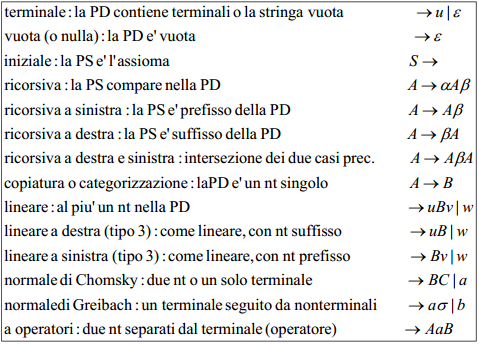
\includegraphics[width=0.6\linewidth]{img/tipiregole.png}
	\caption{Tipi di regole}\label{fig:tipiregole}
\end{figure}
\subsection{Derivazione e generazione del linguaggio}
Derivare un linguaggio da un insieme di regole significa procedere nel seguente modo:
$$\beta,\gamma \in (V\cup\Sigma)^*$$
allora $ \gamma $ deriva da $ \beta $ nella grammatica $ G $ 
$$ \beta \Rightarrow \gamma \text{ se } A\rightarrow \alpha \text{ è una regola della grammatica } G$$
ed inoltre
$$\beta = hAd, \ \gamma = h\alpha d$$
Il linguaggio generato da $ G $ quado si parte dal non terminale \emph{A} viene chiamato $ L_A(G) $. Una forma generata da \emph{G} partendo dal non terminale $ A \in V $ è una stringa $ \alpha \in (V\cup \Sigma)^*$ tale che:
$$A\xRightarrow{*}\alpha$$
Se il non terminale \emph{A} è l'\emph{assioma} allora la forma generata è detta frasale. Se la forma frasale generata contiene solamente caratteri terminali allora si chiama semplicemente \emph{frase}.\\
Analizziamo ora l'esempio di una grammatica $ G_I $ che genera la struttura di un libro, il quale contiene un frontespizio $ f $ una serie di uno o più capitoli \emph{A} ed ogni capitolo inizia con un titolo \emph{t} e contiene una o più righe \emph{l}.
La sintassi di questa grammatica è:
$$
\begin{array}{lcl}
S & \rightarrow & fA\\
A & \rightarrow & AtB | tB\\
B & \rightarrow & lB | l\\
\end{array}
$$
Il non terminale \emph{A} genera la forma $ tBtB $ ed eventualmente le stringhe $ tlltl \in L_A(G_I) $. Il non terminale \emph{S}genera forme frasali del tipo $ fAtlB $ e $ FtBtB $.
Un linguaggio si definisce \emph{libero dal contesto} se e solo se esiste una grammatica libera che lo  genera.
In questo esempio il linguaggio generato è anche regolare ma la famiglia di linguaggi liberi \texttt{LIB} contiene strettamente la famiglia di quelli regolari.
$$REG\subset LIB$$
Due grammatiche $ G $ e $ G' $ si dicono \emph{equivalenti} se e solo se generano lo stesso linguaggio, ovvero se $ L(G) = L(G') $
\subsection{Grammatiche errate e regole inutili}
Quando scriviamo una grammatica dobbiamo prestare attenzione che tutti i simboli non terminali siano definiti e tutti questi contribuiscano a generare la stringa del linguaggio. 
Una grammatica si dice in \emph{forma ridotta} se entrambi le condizioni seguenti sono soddisfatte:
\begin{itemize}
\item ogni non-terminale \emph{A} è raggiungibile dall'assioma, ovvero esiste una derivazione come la seguente:
$$S \xRightarrow{*} \alpha A\beta$$
\item Ogni non terminale \emph{A} genera un insieme di stringhe non vuoto.
$$L_A(G) \neq \varnothing$$
\end{itemize}
Per fare ciò si può applicare un algoritmo in due fasi. La prima fase identifica i non terminali non identificati, la seconda fase invece identifica quelli irraggiungibili.\\
Più in dettaglio la fase uno si svolge lungo i seguenti passi:
\begin{itemize}
\item Costruzione dell'insieme complemento \texttt{DEF}	dei non-terminali definiti:
$$DEf = V\setminus UNDEF$$
\item Per costruire tale insieme si inseriscono tutti i non terminali che nelle loro regole presentano nella parte destra solo elementi terminali.
$$DEF:= \{A|(A\rightarrow u)\in P \wedge u\in \Sigma^* \}$$
\item Infine si inseriscono ricorsivamente nell'insieme tutti i non terminali che nelle loro regole presentano nella parte destra dei simboli terminali oppure dei simboli non terminali già inclusi in \texttt{DEF}
$$DEF:= DEF \cup \{B| (B\rightarrow D_1D_2\dots D_n)\in P \}$$
\end{itemize}
Per ogni interazione della prima fase possono accadere due cose, la prima è che viene individuato un nuovo simbolo non terminale da inserire nell'insieme \texttt{DEF} la seconda è che l'insieme \texttt{DEF} non cambia, in questo caso significa che si è raggiunta la convergenza. I simboli non terminali rimasti fuori dall'insieme \texttt{DEF} possono essere eliminati.\\
La seconda fase identifica i non terminali che sono raggiungibili dall'assioma $ S $, questo problema si può ridurre a trovare l'esistenza di un percorso all'interno del grafo costruito tramite la relazione:
$$A\xrightarrow{produce} B \iff A\rightarrow \alpha B\beta \text{ con } A\neq B$$
I non-terminali non raggiungibili possono essere eliminati dalla grammatica.\\
Una terza proprietà può essere applicata per ridurre ulteriormente una grammatica. Questa proprietà definisce che una grammatica \emph{G} non deve avere derivazioni circolari, le quali non sono essenziali e possono portare ad ambiguità.\\
\subsection{Ricorsione e linguaggi infiniti}
La maggior parte dei linguaggi che ci interesseranno sono infiniti, ovvero contengono un numero infinito di stringhe. Ci dobbiamo chiedere quale sia il meccanismo che permetta ad una grammatica libera di generare un'infinità di stringhe. La risposta a questa domanda è la \emph{ricorsione}.
$$A\xRightarrow{n}xAy \quad n\geq 1$$
Condizione necessaria e sufficiente perché un linguaggio $ L(G) $ sia infinito è che la grammatica generativa $ G $ si ricorsiva.
\subsection{Derivazione canonica e albero della sintassi}
Un \emph{albero della sintassi} è un grafo aciclico nel quale ogni coppia di nodi e connessa da uno e un solo percorso non necessariamente diretto. L'albero della sintassi rappresenta graficamente il processo di derivazione, esiste una relazione \emph{padre-figlio} o anche \emph{radice-foglia} tra i nodi. L'insieme di tutte le foglie lette da destra a sinistra è detto \emph{frontiera}. Si definisce \emph{grado} di un nodo (o anche \emph{arità}) il numero di figli di quel nodo.\\
Un \emph{sotto-albero} con radice \emph{N} è l'albero che ha come radice \emph{N} ed include tutti i discendenti di tale nodo. Nel caso di albero della sintassi la radice è l'\emph{assioma} della grammatica e la frontiera è una delle stringhe generate.
Vediamo ora una grammatica in \figurename \ref{fig:gramex} e i corrispettivi sotto-alberi che rappresentano le diverse regole \figurename \ref{fig:subtree}.
\begin{figure}
	\centering
	\subfigure[]
	{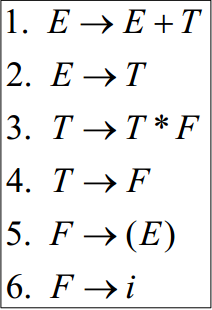
\includegraphics[width=0.25\linewidth]{img/gramex.png}\label{fig:gramex}}
	\hspace{10mm}
	\subfigure[]
	{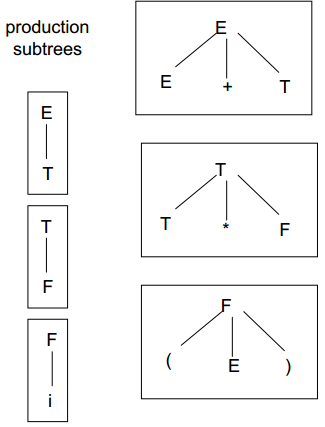
\includegraphics[width=0.3\linewidth]{img/subtree.png}\label{fig:subtree}}
	\caption{Grammatica \ref{fig:gramex} e corrispettivi sotto alberi \ref{fig:subtree}}
\end{figure}

Da questa grammatica possiamo generare diverse stringhe e ad ogni stringa generata possiamo creare un albero sintattico come quello mostrato in \figurename \ref{fig:sintree}, quest'albero lo possiamo rappresentare in versione parentisizzata come segue:
$$[[[[i]_F]_T]_E+[[[i]_F]_T\times [i]_F]_T]_E$$
\begin{figure}
	\centering
	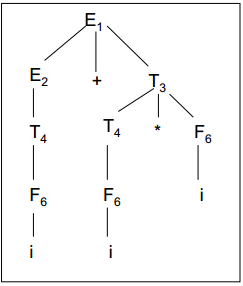
\includegraphics[width=0.32\linewidth]{img/sintree.png}
	\caption{Albero sintattico per la grammatica di \figurename \ref{fig:gramex}}\label{fig:sintree}
\end{figure}
Molte volte quello che conta è solamente la struttura dell'albero e la sua frontiera e non i nodi intermedi per questo si può prendere in considerazione l'\emph{albero scheletrico} come quello di \figurename \ref{fig:skeletont}. 
\begin{figure}
	\centering
	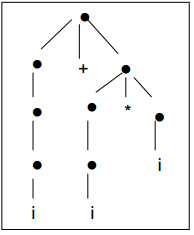
\includegraphics[width=0.32\linewidth]{img/skeletont.png}
	\caption{Albero scheletrico}\label{fig:skeletont}
\end{figure}
Oppure la sua versione condensata nella quale i percorsi lineari come quelli generati dalle regole \emph{2,4,6} vengono collassati.\\
Si parla di \emph{derivazione destra (sinistra)} quando in un albero di derivazione si deriva prima il nodo di frontiera più a \emph{destra (sinistra)} ovvero in una frase di non terminali come quella in esempio si applica la derivazione seguente
$$E+T\xRightarrow{d}E+T\times F$$
Ogni frase di una grammatica libera può essere generata tramite una derivazione destra o sinistra. Questa proprietà è di grande importanza per gli  algoritmi di analisi sintattica.\\
Frequentemente i linguaggi artificiali contengono strutture innestate come le parentesi, in questo caso si hanno sempre due elementi uno di apertura e uno di chiusura i quali racchiudono alcune sotto strutture tra cui anche altre coppie di elementi innestati, questo può avvenire in modo ricorsivo anche più volte. Se non consideriamo i simboli marcatori per l'apertura e la chiusura ma utilizziamo simboli generici come le parentesi il linguaggio che otteniamo è detto \emph{linguaggio di Dyck}. Le frasi generate da questo linguaggio possono essere definite equivalentemente tramite le \emph{regole di cancellazione} che consistono nella cancellazione di copie adiacenti di tag apertura e chiusura. La stringa originale si definisce valida se il risultato finale della cancellazione è la \emph{stringa vuota}.\\
Le operazioni regolari di base, ovvero \emph{unione, concatenazione e stella} applicati ai linguaggi liberi danno come risultato altri linguaggi liberi. Ciò significa che i linguaggi liberi sono chiusi rispetto a queste operazione.
\begin{itemize}
	\item Unione
	$$G= (\Sigma_1 \cup \Sigma_2, \{S\}\cup V_{N_1} \cup V_{N_2}, \{S \rightarrow S_1|S_2 \} \cup P_1\cup P_2, S)$$
	\item Concatenazione
	$$G= (\Sigma_1 \cup \Sigma_2, \{S\}\cup V_{N_1} \cup V_{N_2}, \{S \rightarrow S_1S_2 \} \cup P_1\cup P_2, S)$$
	\item Stella: tale grammatica è ottenuta aggiungendo la regola 
	$$S\rightarrow SS_1 | \varepsilon$$
\end{itemize}
Tuttavia per applicare queste regolo è necessario che gli insiemi dei non terminali siano disgiunti e che il nuovo assioma non appartenga all'unione dei due insiemi di non terminali.
$$ V_{N_1}\cap V_{N_2} = \varnothing \quad S \notin ( V_{N_1}\cup V_{N_2} )$$
La famiglia dei linguaggi liberi \texttt{LIB} è chiusa inoltre rispetto alla riflessione, infatti, per ogni regola della grammatica G basta riflettere la parte destra.
\subsection{Ambiguità}
Esistono diversi tipi ambiguità, una prima distinzione è tra ambiguità \emph{sintattica} e \emph{semantica}. L'ambiguità semantica è quella dovuta al significato del linguaggio come nel caso del linguaggio naturale. Nel caso di linguaggi artificiali tuttavia l'ambiguità semantica è indesiderabile.\\
L'ambiguità sintattica si ha quando  una frase \emph{x} di un linguaggio generato da una grammatica \emph{G} ammette più di un albero sintattico e quindi più derivazioni. Una grammatica \emph{g} si definisce ambigua se ammette anche una sola stringa ambigua.
Un esempio è la grammatica $ G' $ che risulta essere ambigua:
$$E \rightarrow E + E | E\times E| (E)| i$$
La quale genera la stringa $ i+i\times i $ che è ambigua in quanto ammette due alberi sintattici che sono quelli in \figurename \ref{fig:g1tree}
\begin{figure}
\centering
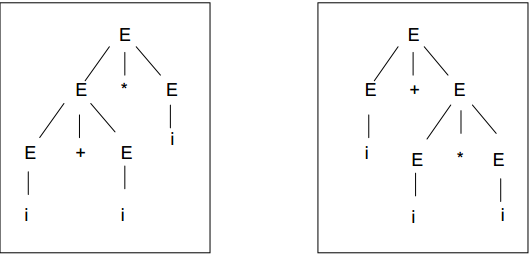
\includegraphics[width=0.5\linewidth]{img/g1tree.png}
\caption{Due alberi sintattici che generano la stessa stringa}\label{fig:g1tree}
\end{figure}
Si definisce \emph{grado di ambiguità} di una frase \emph{x} il numero di differenti alberi sintattici che generano la stringa \emph{x}. Il \emph{grado di ambiguità} di una \emph{grammatica} è il grado massimo di ambiguità di una stringa \emph{x} tra tutte quelle generate dalla grammatica.
Decidere se una grammatica è ambigua è un problema \emph{indecidibile} quindi non esiste un algoritmo per determinare se una grammatica è ambigua oppure no. Tuttavia per alcune grammatiche è possibile esplorare tutti i grafi e quindi stabilire se una determinata grammatica è ambigua; è quindi  auspicabile che la non ambiguità di una grammatica sia determinata in fase di costruzione.\\
Se un simbolo non terminale è ricorsivo sia a destra che a sinistra solitamente permette due o più modi di derivazione e questo porta sempre ad un comportamento ambiguo.\\
Se due linguaggi $ L_1(G_1) $ e $ L_2(G_2) $ condividono alcune frasi, ovvero la loro intersezione non è vuota la grammatica che risulta come unione delle due è sicuramente ambigua on quanto esiste un albero in $ G_1 $ e uno in $ G_2 $.\\
Esistono poi dei linguaggi che sono \emph{internamente} ambigui e di conseguenza tutte le grammatiche che generano questi linguaggi sono ambigue. Consideriamo ad esempio il linguaggio 
$$L = \{a^ib^jc^k | (i,j,k\geq 0) \wedge ((i=j)\vee (j= k) \}$$
In quanto possiamo suddividerlo in due linguaggi ed effettuarne l'unione.
$$L = \{a^ib^ic^* |i \geq 0 \} \cup \{a*ib^jc^j |j \geq 0 \}= L_1 \cup L_2$$
In questo caso tutte le stringhe del tipo $ \varepsilon,abc,a^2b^2c^2,\dots $ sono generabili in entrambi i linguaggi. Questo comportamento è dovuto alla natura del linguaggio e in qualsiasi modo si modifichino le grammatiche che generano il comportamento delle frasi, l'ambiguità è inevitabile.\\
La concatenazione di due linguaggi può portare ambiguità se essiste un suffisso di una frasedel primo linguaggio che è anche prefisso di una frase del secondo linguaggio.
	$$G= (\Sigma_1 \cup \Sigma_2, \{S\}\cup V_{N_1} \cup V_{N_2}, \{S \rightarrow S_1S_2 \} \cup P_1\cup P_2, S)$$
Assumiamo che le grammatiche $ G_1 $ e $ G_2 $ non siano ambigue, allora $ G $ è ambigua se esistono due frasi $ x' \in L_1 $ e $ x'' \in L_2 $ ed una stringa non vuota $ v $ tale che:
$$x' = u'v \vee u'\in L_1 \quad x'' = vz'' \vee z'' \in L_2$$
Allora la stringa:
$$u'vz''\in L_1\cdot L_2$$
è ambigua infatti le due derivazioni sono:
$$
\begin{array}{ccccccc}
S & \Rightarrow & S_1S_2 & \xRightarrow{+} & u'S_2 & \xRightarrow{+} & u'vz''\\
S & \Rightarrow & S_1S_2 & \xRightarrow{+} & u'vS_2 & \xRightarrow{+} & u'vz''
\end{array}
$$
\subsection{Equivalenza forte ed equivalenza debole}
Due grammatiche $ G $ e $ G' $ si definiscono debolmente equivalenti se e solo se generano lo stesso linguaggio ovvero se $ L(G) = L(G') $. Queste due grammatiche possono avere strutture (alberi sintattici) completamente diversi per generare la stessa frase, può capitare perciò che alcune strutture siano inadeguate per alcuni usi.\\
L'equivalenza \emph{forte} o \emph{strutturale} si ha quando due grammatiche $ G $ e $ G' $ generano lo stesso linguaggio e per ogni frase hanno alberi sintattici equivalenti ovvero l'albero scheletrico condensato è identico per entrambe le grammatiche. L'equivalenza forte implica quella debole ma non viceversa, inoltre l'equivalenza forte è una proprietà decidibile, mentre quella debole non lo è.\\
Quando si definisce formalmente un linguaggio non si può fare a meno di tenere in considerazione un'\emph{adeguatezza strutturale}, in quanto la grammatica generata dal linguaggio è la base sintattica per definire l'interpretazione semantica delle frasi.\\
Esiste poi quella che viene definita \emph{equivalenza strutturale in senso largo}. Consideriamo due grammatiche come le seguenti:
$$\{S\rightarrow Sa|a\} \quad \{X\rightarrow aX | a \} $$
Queste due grammatiche non sono equivalenti strutturalmente in quanto per generare la stringa $ aa $ creano due alberi sintattici diversi, tuttavia l'unica differenza che intercorre tra le due è che l'albero sintattico della seconda è rispecchiato rispetto alla prima. Si dice quindi che le due grammatiche sono equivalenti in senso \emph{largo}.
\subsection{Grammatiche in forma normale}
Una grammatica in forma normale comporta alcune restrizioni a livello di regole, tuttavia non ne limita la potenza espressiva. Questo tipo di forma è utile per dimostrare i teoremi piuttosto che per la definnizioni di linguaggi.\\
Esistono alcune trasformazioni per trasformare una grammatica dalla sua forma generale alla sua forma normale. Queste trasformazioni sono utili per costruire degli analizzatori sintattici.
\paragraph{Espansione di un non terminale}
Prendiamo in considerazione la grammatica $ G = \{\Sigma,V,P,S \} $ composta dalle seguenti due regole
$$A\rightarrow \alpha B \gamma \quad B\rightarrow \beta_1|\beta_2|\dots|\beta_n$$
L'espansione di un simbolo non terminale significa sostituire un non terminale in una regola in modo da eliminarlo come in questo caso possiamo fare con il non terminale $ B $.
$$A\rightarrow \alpha\beta_1\gamma|\alpha\beta_2\gamma|\dots|\alpha\beta_n\gamma$$
\paragraph{Rimozione dell'assioma dalla parte destra}
È sempre possibile limitare la parte destra di una regola al solo alfabeto $ (\Sigma \cup (V-\{S\})) $ ovvero è sempre possibile eliminare l'assioma dalle parti destre delle regole, è sufficiente introdurre un nuovo assioma $ S_0 $ e la corrispettiva regola $ S_0\rightarrow S $
\paragraph{Non-terminali annullabili}
Un non-terminale si dice \emph{annullabile} se e solo se esiste una derivazione come la seguente
$$A\xRightarrow{+}\varepsilon$$
Questo tuttavia non significa che il non terminale in questione possa generare altre stringhe diverse da $ \varepsilon $.
Consideriamo $ Null\subseteq V $ l'insieme dei non terminali annullabili allora
$$A \in Null \iff (A\rightarrow \varepsilon \in P9 \wedge ((A\rightarrow A_1A_2\dots A_n \in P \ con \ A_i\in V\backslash\{A\})\wedge \forall A_i (A_i \in Null))$$
Un esempio è la grammatica:
$$S\rightarrow SAB | AC \quad A\rightarrow aA|\varepsilon \quad B\rightarrow bB|\varepsilon \quad C\rightarrow cC|c$$
L'insieme dei non-terminali annullabili è 
$$Null= \{ A,B\}$$
Una grammatica si dice in forma \emph{non annullabile} se e solo se contiene tutti non-terminali non annullabili e l'assioma è annullabile se e solo se il linguaggio contiene la stringa vuota $S\rightarrow \varepsilon$.\\
Per ottenere una grammatica in forma normale non annullabile dobbiamo procedere lungo i seguenti passi:
\begin{enumerate}
	\item Calcolare l'insieme \emph{Null}
	\item Per ogni regola di \emph{P} aggiungere una regola ottenuta da quelle di \emph{P} eliminando ogni non-terminale annullabile che si presenta nella parte destra delle regole in ogni sua forma.
	\item Eliminare le regole vuote del tipo $ A\rightarrow \varepsilon $ a meno che non sia $ A=S $
	\item Rimuovere $ S\rightarrow \varepsilon $ se e solo se il linguaggio non contiene la stringa vuota.
	\item Portare la grammatica in forma ridotta rimuovendo le derivazioni circolari.
\end{enumerate}
\subsection{Regole di copiatura e loro eliminazione}
Prendiamo ad esempio la regola $A\rightarrow B$, in questa regola la classe sintattica $ B $ è inclusa in quella di \emph{A}, rimuovendola si ottiene una grammatica equivalente ma che ha un albero sintattico meno profondo.
Consideriamo ora $ Copy(A)\subseteq V $ come l'insieme dei non-terminali in cui il terminale \emph{A} viene copiato. Le regole di copiatura non sono totalmente inutili anzi talvolta ci permetono di condividere alcune parti della grammatica, per questo le regole di copiatura vengono utilizzate nelle grammatiche dei linguaggi tecnici come ad esempio le istanze nei linguaggi di programmazione.\\
Per eliminare le regole di copiatura per prima cosa dobbiamo calcolare l'insieme \emph{Copy}; per calcolare tale insieme si seguono le seguenti clausole logiche.
$$A \in Copy(A)$$
$$C \in Copy(A) \ se \ (B\in Copy(A))\wedge (B\rightarrow C \in P)$$
A questo punto si costruisce la grammatica $ G' $ equivalente a $ G $ ma senza le regole di copiatura.
\subsection{Forma normale di Chomsky}
Nella forma normale di Chomsky abbiamo solo due tipi di regole:
\begin{itemize}
	\item Regole binarie:
	$$A\rightarrow BC \ dove \ B,C \in V$$
	\item Regole terminali, con una sola lettera sul lato destro:
	$$A \rightarrow a \ dove \ a\in\Sigma$$
\end{itemize}
Se il linguaggio contiene la stringa vuota è  necessario aggiungere la regola:
$$S\rightarrow \varepsilon$$
Un esempio di trasformazione in forma normale di Chomsky è mostrato in \figurename \ref{fig:chomsky} dove i simboli tra parentesi angolari ($ < > $) indicano dei simboli non-terminali introdotti appositamente.
\begin{figure}
	\centering
	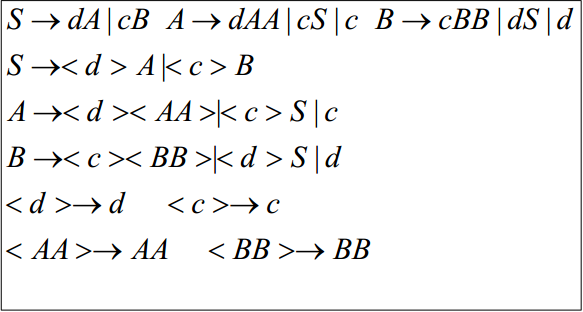
\includegraphics[width=0.5\linewidth]{img/chomsky.png}
	\caption{Esempio di trasformazione in forma normale di chomsky}\label{fig:chomsky}
\end{figure}
\subsection{Forma normale \emph{Real Time}}
Prima di introdurre la forma normale real time dobbiamo introdurre la \emph{trasformazione della ricorsione sinistra} in una ricorsione destra. Prima di tutto si parte con il trasformare una ricorsione sinistra in una forma non ricorsiva a sinitra come nell'esempio mostrato in \figurename \ref{fig:leftrec} questa trasformazione è indispensabile per creare anallizzatori sintattici discendenti.
\begin{figure}
	\centering
	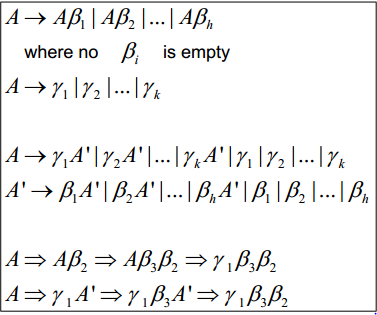
\includegraphics[width=0.4\linewidth]{img/leftrec.png}
	\caption{Esempio di trasformazione di una ricorsione sinistra}\label{fig:leftrec}
\end{figure}
In questo esempiio la ricorsione è diretta, tuttavia nel caso la ricorsione non sia diretta si lavora con un algoritmo in due fasi che però necessita di alcune ipotesi, ovvero, la grammatica \emph{G} deve essere non-omogenea, non-annullabile e le regole devono presentare al massimo un non terminale. L'algoritmo applicato lavora iterativamente su due passi, il primo consiste nell'espansione delle regole per esporre la ricorsione sinistra, il secondo passaggio trasforma la ricorsione sinistra in una ricorsione destra.
La forma \emph{normale real-time} è una forma nella quale le regole della grammatica iniziano sempre con un simbolo terminale (niente ricorsione sinistra). 
$$A\rightarrow a\alpha \ dove \ a \in \Sigma, \alpha\in\{\Sigma\cup V \}^*$$
Esiste poi una particolare forma real time che è quella di \emph{Greibach} nella quale il simbolo terminale è seguito da uno o più non-terminali.
$$A\rightarrow a\alpha \ dove \ a \in \Sigma, \alpha\in V^*$$
Il termine \emph{real time} viene utilizzato perché l'analizzatore sintattico costruito con questo tipo di grammatiche analizza e consuma un solo carattere terminale ad ogni step e quindi l'algoritmo impiega tanti step quanto è la lunghezza della stringa.\\
Per trasformare una grammatica in forma normale real time bisogno che essa sia non-annullabile e si procede nei seguenti passi:
\begin{itemize}
	\item Si elimina la ricorsione diretta, sia immediata che non \figurename \ref{fig:rt1}
	\item Mediante trasformazioni elementari, si espandono i non-terminali più a sinistra della parte destra della regola \figurename \ref{fig:rt2}
	\item Si introducono nuovi non-terminali per eliminare eventuali simboli terminali che si presentano all'estremità destra della parte destra della regola \figurename \ref{fig:rt3}. 
\end{itemize}

\begin{figure}
	\centering
	\subfigure[]{
		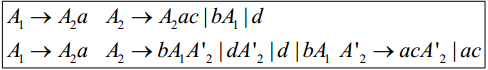
\includegraphics[width=0.4\linewidth]{img/rt1.png}\label{fig:rt1}
	}
	\subfigure[]{
		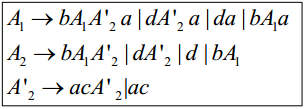
\includegraphics[width=0.3\linewidth]{img/rt2.png}\label{fig:rt2}
	}
	\subfigure[]{
		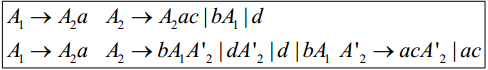
\includegraphics[width=0.4\linewidth]{img/rt1.png}\label{fig:rt3}
	}
	\caption{Esempio di trasformazione in forma normale}
\end{figure}
\subsection{Linguaggi regolari e grammatiche libere}
I linguaggu regolari sono casi particolari di quelli liberi, essi infatti possono essere generati da gramatiche che presentano delle regole fortemente ristrette. Man mano che la lunghezza di una stringa generata da un linguaggio regolare cresce essa presenta delle sottostringhe ripetute.\\
È possibile dimostrare in modo rigoroso che alcuni linguaggi liberi non possono essere generate da espressioni regolari.
Nei linguaggi regolari per identificare una stringa è necessaria solo una quantità finita di memoria, per i linguaggi liberi invece la quantità di memoria deve essere infinita.
\subsubsection{Dalle espressioni regolari alle grammatiche libere}
Gli operatori iterativi regolari come \emph{stella} e \emph{croce} posso essere sostituiti da regole ricorsive. Per fare ciò si dividono le espressioni regolari in sotto-espressioni e si enumerano progressivamente, dopo aver fatto questo si trasformano le \emph{regexp} utilizzando le trasformazioni di \figurename \ref{fig:regtogram}.
\begin{figure}
	\centering
	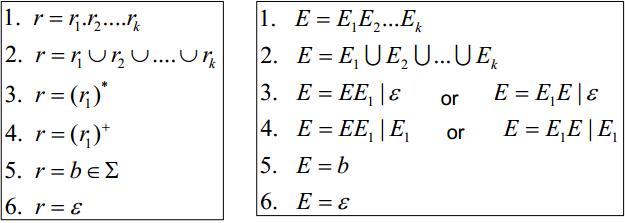
\includegraphics[width=0.5\linewidth]{img/regtogram.png}
	\caption{Regole di trasformazione da \emph{regexp} a grammatica libera}\label{fig:regtogram}
\end{figure}
Nel caso la in cui l'espressione regolare risulti ambigua anche l'equivalente grammatica sarà ambigua. Ogni linguaggio regolare è libero ma non tutti i linguaggi liberi sono regolari.
$$REG \subset LIB$$
\subsubsection{Grammatiche lineari}
Una grammatica si definisce lineare se ogni regola ha al più un non-terminale nella parte destra della regola.
$$A\rightarrow uBv \text{ dove } u,v \in \Sigma^*, B\in (V\cup\varepsilon)$$
%\include{capitolo4}
%\include{capitolo5}
%\include{capitolo6}
%\include{capitolo7}
%\include{capitolo8}
%\include{capitolo9}

\newpage
\listoffigures

\end{document}